\documentclass[tikz,border=1.5mm]{standalone}
\usepackage{graphicx}
\usepackage{tikz}
\usetikzlibrary{arrows.meta,calc,positioning,shapes.geometric}
\definecolor{r19blue}{HTML}{1F5A85}
\definecolor{r19teal}{HTML}{287C7B}
\definecolor{r19red}{HTML}{B84537}
\definecolor{r19ink}{HTML}{263238}
\definecolor{r19paper}{HTML}{FFFFFF}
\begin{document}
\begin{tikzpicture}[x=1cm,y=1cm,font=\sffamily]
\node[anchor=south west,inner sep=0] at (0,0){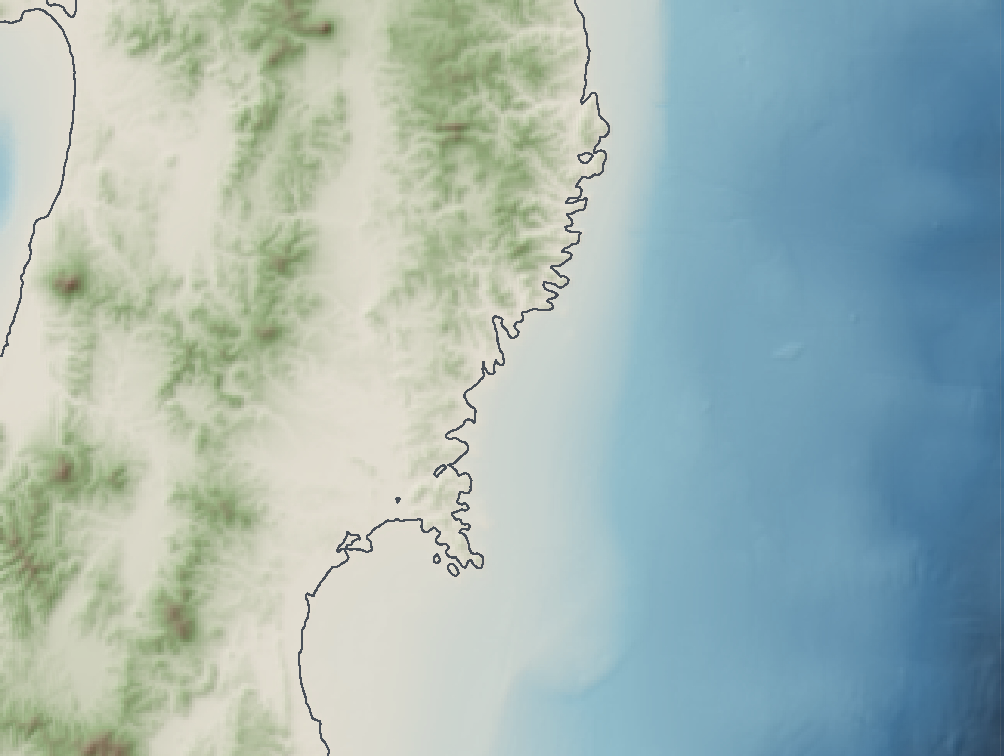
\includegraphics[width=16.0000cm,height=12.0615cm]{../qgis/T1_qgis_base.pdf}};
\fill[r19blue!28,fill opacity=0.42] (11.1739,2.4248) -- (11.5391,2.5723) -- (9.2654,8.2016) -- (8.9002,8.0541) -- (11.1739,2.4248) -- cycle;
\draw[r19blue,line width=1.05pt] (11.1739,2.4248) -- (11.5391,2.5723) -- (9.2654,8.2016) -- (8.9002,8.0541) -- (11.1739,2.4248) -- cycle;
\draw[r19blue,densely dashed,line width=0.85pt] (11.3565,2.4986) -- (9.0828,8.1278);
\draw[r19teal,line width=1.05pt] (10.2886,5.6684) -- (9.9234,5.5209);
\draw[{Latex[length=2.2mm]}-{Latex[length=2.2mm]},r19blue,line width=0.72pt] (10.7630,2.2589) -- (8.4894,7.8881) node[midway,sloped,above=2pt,fill=r19paper,inner sep=1.7pt,text=r19ink]{$L_c=123.319\,\mathrm{km}$};
\draw[{Latex[length=2.0mm]}-{Latex[length=2.0mm]},r19teal,line width=0.72pt] (10.2886,5.6684) -- (9.9234,5.5209) node[midway,sloped,above=2pt,fill=r19paper,inner sep=1.5pt,text=r19ink]{$W_c=8.000\,\mathrm{km}$};
\node[circle,draw=r19red,fill=r19red,inner sep=1.9pt,label={[fill=r19paper,inner sep=1.3pt,text=r19ink]20:USGS 2011 event ref.}] at (11.0799,3.1833) {};
\node[circle,draw=r19ink,fill=r19paper,inner sep=1.8pt,label={[fill=r19paper,inner sep=1.3pt,text=r19ink]80:Kamaishi proxy}] at (8.9307,8.5044) {};
\node[diamond,draw=r19teal,fill=r19teal,inner sep=1.9pt,label={[fill=r19paper,inner sep=1.3pt,text=r19ink]5:selected wet interface}] at (9.0828,8.1278) {};
\node[circle,draw=r19blue,fill=r19paper,inner sep=1.3pt,label={[fill=r19paper,inner sep=1.2pt,text=r19ink]180:source-side boundary}] at (11.3565,2.4986) {};
\node[anchor=west,fill=r19paper,fill opacity=0.90,text opacity=1,inner sep=2.2pt,text=r19ink] at (0.45,11.4815) {\begin{tabular}{@{}l@{}}Regional2D delivery corridor\\$L_{prop}=108.319\,\mathrm{km}$ event to interface\\$L_{pre}=15.000\,\mathrm{km}$, $L_{inland}=0$\end{tabular}};
\draw[-{Latex[length=2.5mm]},r19ink,line width=0.82pt] (14.9500,10.2115) -- ++(0,1.00) node[above]{N};
\draw[-{Latex[length=2.2mm]},r19red,line width=0.82pt] (14.9500,10.2115) -- ++(-0.38,0.92);
\node[anchor=east,fill=r19paper,fill opacity=0.88,text opacity=1,inner sep=1.6pt,text=r19ink] at (14.8000,11.0115) {$\theta_c=338.0^\circ$ cw\\($22.0^\circ$ W of N)};
\draw[r19ink,line width=1.45pt] (0.65,0.48) -- ++(2.4615,0);
\draw[r19ink,line width=0.65pt] (0.65,0.39) -- (0.65,0.57) (3.1115,0.39) -- (3.1115,0.57);
\node[anchor=north,text=r19ink,fill=r19paper,fill opacity=0.86,text opacity=1,inner sep=1pt] at (1.8808,0.34) {50 km};
\end{tikzpicture}
\end{document}
